% Requires running Bibtex

\documentclass[%
reprint,
amsmath,amssymb,
aps,
floatfix
]{revtex4-2}

\usepackage{graphicx}% Include figure files
\usepackage{dcolumn}% Align table columns on decimal point
\usepackage{bm}% bold math
\usepackage{hyperref}% add hypertext capabilities
\usepackage[font=scriptsize,labelfont=bf, justification=justified]{caption}% change fontsize in captions
\usepackage{float}
\usepackage{booktabs}% cool table style
\hypersetup{
	colorlinks=true,       % false: boxed links; true: colored links
	linkcolor=black,        % color of internal links
	citecolor=black,        % color of links to bibliography
	filecolor=black,     % color of file links
	urlcolor=black         
}

\usepackage{listings}

%\usepackage{bibspacing}
%\setlength{\bibitemsep}{.5\baselineskip plus .05\baselineskip minus .05\baselineskip}


\begin{document}
	
	\preprint{APS/123-QED}
	
	\title{PHYC30170 Physics with Astronomy and Space Science Lab 1;\\An Investigation of the Ramsauer-Townsend Effect}
	
	\author{Daragh Hollman}
	\email{daragh.hollman@ucdconnect.ie}
	
	\date{\today}
	\maketitle
	
	\section{Introduction}
	What is the Ramsauer-Townsend effect? ; What are it's applications?\\
	
	The Ramsauer-Townsend effect describes the phonomenon where electrons exhibit a minimum scattering cross section around electron energies of $1\,\text{eV}$ in nobel gases \cite{wisconsin}. This interaction between particles cannot be described by a classical interpretation of particle collisions and requires a quantum mechanical description \cite{texas}. It is important to understand and experimentally test the Ramsauer-Townsend effect as to better understand how particle colloissions work in quantum mechanics.
	
	\section{Theory}
	Why and how does the effect happen? talk about scattering, contact potentials...
	
	Explain scattering. The hard sphere model of particle collissions cannot be used, a quantum mechanicical model must be use. Explain what we would see classically and what we would see quantum mechanically.\\
	
	Under classical mechanics, scattering particles are described by hard sphere scattering, where particles collide and interact as billard balls might. Such a model is described in figure \ref{fig:hardSphereScattering} where the potential experienced by a light scattered particle is $U(r) = 0$ for $r > R$ and $U(r) = \infty$ for $r < R$ where $R$ is the radius of the sphere it scatters off \cite{santaBarbara}. It follows that, for a projectile particle moving towards the target but offset by a distance from the axis greater than $R$, the particle would not be deflected at all. We see there is some region with which the scattered particle cannot pass through, this area is known as the scattering cross section and when with respect to the total area it is analgous to the probability of scattering \cite{santaBarbara}.\\
	
	\begin{figure}
		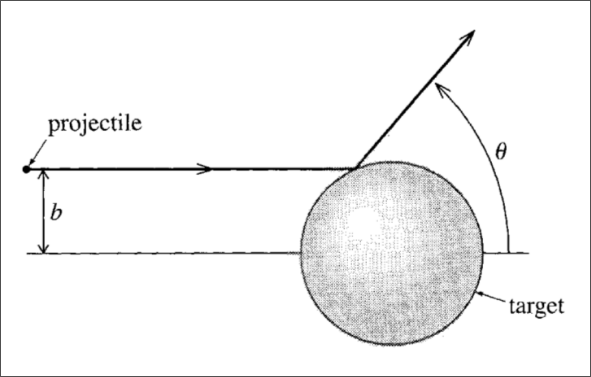
\includegraphics[width=0.85\columnwidth]{hardSphereScattering.png}
		\caption{\label{fig:hardSphereScattering}A simple hard sphere scattering model described by the potential $U(r) = 0$ for $r > R$ and $U(r) = \infty$ for $r < R$}
	\end{figure}
	
	When considered in this way, the scattering cross section of the nobel gas atoms is independent of the incident electron energy. However, if the noble gas atoms are treated within quantum mechanics and present an attractive potential, akin to a square well, the solution of Schrödinger's equation yields that the scattering cross section will have a minimum for electron energies near $1 \,\text{eV}$ \cite{kukolich} \cite{sobhani}. The scattering of electrons by a square well can be predicted by a one-dimensional model or a three-dimensional model \cite{kukolich}. These models represent the xenon atom as a square well with positive potential.
	
	\section{Methodology}
	\subsection{Apparatus Setup}
	
	
	\section{Results \& Analysis}
	Present inital results of the minium point and after include diagram of contact potential and include that to have a final measurement. Note that although a excitation voltage of up to 6 volts could be used, a lower choice of 4 volts was used to reduce the temperature of the filament and hence reduce the spread of electron energies.
	
	\section{Conclusion}
		
	\clearpage
	\bibliography{ramsauer.bib}% Produces the bibliography via BibTeX.
	
	\clearpage
	\onecolumngrid
	\appendix


	
	
\end{document}

